\documentclass{beamer}
% imprimir
% \documentclass[handout]{beamer} 
% \usepackage{pgfpages}
% \pgfpagesuselayout{4 on 1}[a4paper,landscape,border shrink=5mm]

\mode<presentation> {
  \usetheme{Warsaw}
  \setbeamercovered{transparent}
}

\usebackgroundtemplate{
\includegraphics[width=\paperwidth]{format/libresoft-bg.png}}
\usepackage[spanish]{babel}
\usepackage[utf8]{inputenc}
\usepackage{graphics}
\usepackage{hyperref}
\usepackage{amssymb} % Simbolos matematicos

%\definecolor{libresoftgreen}{RGB}{162,190,43}
%\definecolor{libresoftblue}{RGB}{0,98,143}

%\setbeamercolor{titlelike}{bg=libresoftgreen}

%% Metadatos del PDF.
\hypersetup{  
  pdftitle={Cortafuegos con Packet Filter (PF)},
  pdfauthor={Miguel Vidal},
  pdfcreator={GSyC/Libresoft},
  pdfproducer=PDFLaTeX,
  pdfsubject={Master on Free Software},
}
%%

\begin{document}

\title{Cortafuegos con Packet Filter (PF)}
\subtitle{Curso Arquitectura de Servidores}
\institute{\{mvidal,jfcastro\}@libresoft.es} 
\author{Miguel Vidal, José Castro}
%\date{\today}
\date{29 de abril de 2011}

\frame{
\maketitle
\begin{center}

\includegraphics[width=6cm]{format/gsyc-urjc}
\end{center}
}

%% License slide
\begin{frame}
  \vspace{2cm}
  \begin{flushright}
    {\footnotesize \copyright{} 2011 Miguel Vidal, Jose Castro.} \\
%    \vspace{0.25cm}
    \medskip
    {\scriptsize Esta presentación se distribuye bajo \\ licencia Creative Commons Reconocimiento 3.0 España}
%    \vspace{0.10cm}
  \end{flushright}
  \begin{center}
    \href{http://creativecommons.org/licenses/by/3.0/es}{
\includegraphics[width=2cm]{format/cc-by.png}} \\
    {\tiny \url{http://creativecommons.org/licenses/by/3.0/es}}
  \end{center}
\end{frame}%%


\normalsize

%%%%%%%%%%%%%%%%%%%%%%%%%%%%%%%%%%%%%%%%%%%%%%%%%%%%%%%%%%%%%%%%%%%%%%%
\section{Cortafuegos y filtrado TCP/IP}
%%%%%%%%%%%%%%%%%%%%%%%%%%%%%%%%%%%%%%%%%%%%%%%%%%%%%%%%%%%%%%%%%%%%%%%

\begin{frame}

\begin{center}
\huge{Cortafuegos y filtrado de paquetes}
\end{center}

\end{frame}


%%%%%%%%%%%%%%%%%%%%%%%%%%%%%%%%%%%%%%%%%%%%%%%%%%%%%%%%%%%%%%%%%%%%%%%

\begin{frame}
\frametitle{¿Qué es un cortafuegos? (1)}

\begin{itemize}
\item FW (Firewall): término usado para referirse a cosas muy dispares en los últimos años.
\item Se llama lo mismo al FW casero que te colocan en tu línea ADSL o al que le cuesta miles de dólares en una empresa.
\item ¿Qué diferencias hay?

	\begin{itemize}
	\item Funcionalidades que ofrece.
	\item Hardware en el que corre.
	\item Robustez y fiabilidad de su software.
	\end{itemize}

\end{itemize}
\end{frame}

%%%%%%%%%%%%%%%%%%%%%%%%%%%%%%%%%%%%%%%%%%%%%%%%%%%%%%%%%%%%%%%%%%%%%%%

\begin{frame}
\frametitle{¿Qué es un cortafuegos? (2)}

\begin{itemize}
\item Un equipo protegido y fiable que funciona como punto de regulación entre un grupo de redes (normalmente una red privada y una red pública).
\item Todo el tráfico de red entre las redes involucradas se encamina a través del cortafuegos.
\item En grandes corporaciones incluso puede haber cortafuegos dentro de la red corporativa para aislar las zonas importantes de la organización.
\item Crear cortafuegos es un arte: exige comprender muy bien la tecnología de red subyacente, pero también la filosofía de diseño de cortafuegos.
\end{itemize}

\end{frame}



%%%%%%%%%%%%%%%%%%%%%%%%%%%%%%%%%%%%%%%%%%%%%%%%%%%%%%%%%%%%%%%%%%%%%%%

\begin{frame}
\frametitle{¿Qué es un cortafuegos? (y 3)}

\begin{itemize}
\item Un cortafuegos se configura mediante un conjunto de reglas que determina qué tráfico puede pasar y cuál será bloqueado (con respuesta) o desechado (sin respuesta).
\item Los cortafuegos pueden situarse de formas distintas: 
	\begin{itemize}
	\item La forma más simple (e insegura) es un solo equipo que además proporciona otros servicios.
	\item La forma más sofisticada son las DMZ (o red perimetral), que puede involucrar a varios equipos cortafuegos. 
	\end{itemize}
\end{itemize}

\end{frame}

%%%%%%%%%%%%%%%%%%%%%%%%%%%%%%%%%%%%%%%%%%%%%%%%%%%%%%%%%%%%%%%%%%%%%%%

\begin{frame}
\frametitle{Diseño de cortafuegos con un solo firewall}

\begin{figure}[h]

\begin{center}
  \centering
  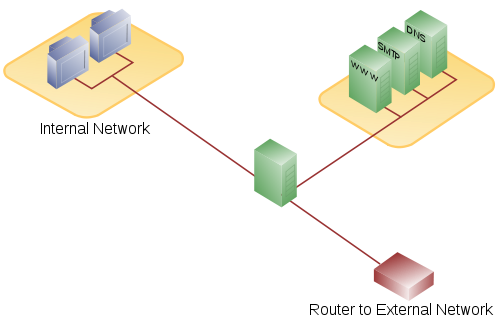
\includegraphics[height=2.7in]{figs/500px-DMZ_network_diagram_1_firewall.png}
  %\caption{Diseño sencillo de UN FW. \textit{Fuente:} Wikipedia.}
\end{center}
\end{figure}

\end{frame}

%%%%%%%%%%%%%%%%%%%%%%%%%%%%%%%%%%%%%%%%%%%%%%%%%%%%%%%%%%%%%%%%%%%%%%%

\begin{frame}
\frametitle{Diseño de cortafuegos con 2 firewalls (DMZ)}

\begin{figure}[h]

\begin{center}
  \centering
  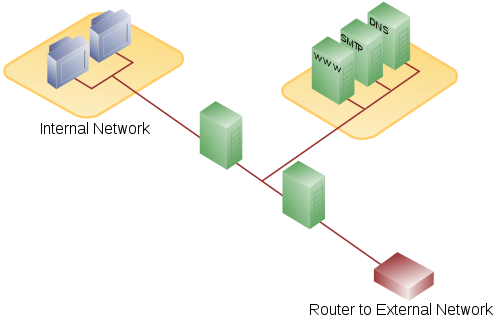
\includegraphics[height=2.7in]{figs/500px-DMZ_network_diagram_2_firewall.png}
%  \caption{2 firewalls. \textit{Fuente:} Wikipedia.}
\end{center}
\end{figure}

\end{frame}


%%%%%%%%%%%%%%%%%%%%%%%%%%%%%%%%%%%%%%%%%%%%%%%%%%%%%%%%%%%%%%%%%%%%%%%

\begin{frame}
\frametitle{Tipos de procesado de paquetes}

\begin{itemize}
\item \alert{Filtrado:} decidir en distintos momentos del flujo si un paquete pasa o es bloqueado.
\item \alert{Modificación:} modificación mientras se mueve el flujo de paquetes
\item \alert{Traducción (NAT)}: permite redirigir el tráfico de forma transparente mediante la modificación de la fuente, el destino o los puertos.
\end{itemize}

\end{frame}

%%%%%%%%%%%%%%%%%%%%%%%%%%%%%%%%%%%%%%%%%%%%%%%%%%%%%%%%%%%%%%%%%%%%%%%

\begin{frame}
\frametitle{¿Qué es el filtrado de IP?}

El filtrado IP consiste en decidir qué paquetes se procesarán y cuáles serán rechazados. Algunos criterios posibles para filtrar:

\begin{itemize}
\item Tipo de protocolo: TCP, UDP, ICMP, etc.
\item Número de puerto (para TCP/UDP)
\item Tipo de paquete: SYN/ACK, datos, petición de eco ICMP...
\item Origen del paquete
\item Destino del paquete
\end{itemize}

Los conjuntos de reglas (\textit{rulesets}) se componen mediante combinación de algunos de estos criterios.

\end{frame}

%%%%%%%%%%%%%%%%%%%%%%%%%%%%%%%%%%%%%%%%%%%%%%%%%%%%%%%%%%%%%%%%%%%%%%%

\begin{frame}
\frametitle{¿Qué es el filtrado de IP?}

\begin{itemize}
\item El filtrado IP es una utilidad de capa de red (layer-3).
\item No conoce nada de las aplicaciones que usan las conexiones de red.
\item Por ejemplo, si filtramos por puerto, ese mismo servicio podría ejecutarse en otro puerto y el firewall no lo impediría.
\item Para solucionar esto, se usan \alert{servidores proxy}, que gestionan la conexión y sí comprenden el servicio.
\end{itemize}

\end{frame}

%%%%%%%%%%%%%%%%%%%%%%%%%%%%%%%%%%%%%%%%%%%%%%%%%%%%%%%%%%%%%%%%%%%%%%%

\begin{frame}
\frametitle{Conceptos básicos}

\begin{itemize}
\item \textit{default accept} versus \textit{default deny}.
\item Inspección de paquetes: \textit{Stateful} vs \textit{stateless}  
\item En los FW de primera generación no habia estado, lo que facilitaba el \textit{spoofing}.
\item La inspección de estado guarda registros de todas las conexiones de red que pasan por el cortafuegos.
\item Establecimiento de la comunicación TCP en tres pasos (\textit{Three-way handshake}):

\begin{itemize}
	\item \alert{SYN packet}: solicitud de sincronización
	\item \alert{SYN+ACK packet}: sincronización y acuse de recibo del servidor
	\item \alert{ACK packet}: acuse de recibo (\textit{acknowledgment}) del cliente.
\end{itemize}

\end{itemize}

\end{frame}


%%%%%%%%%%%%%%%%%%%%%%%%%%%%%%%%%%%%%%%%%%%%%%%%%%%%%%%%%%%%%%%%%%%%%%%

\begin{frame}
\frametitle{Filtrado de paquetes}

\begin{itemize}
\item Un firewall avanzado puede hacer más cosas además de bloquear. 
\item Realiza otras funcionalidades importantes: enmascaramiento, NAT, auditorías, gestión de ancho de banda, balanceo de carga, filtrado por criterios específicos, redundancia...
\end{itemize}

\end{frame}

%%%%%%%%%%%%%%%%%%%%%%%%%%%%%%%%%%%%%%%%%%%%%%%%%%%%%%%%%%%%%%%%%%%%%%%

\begin{frame}
\frametitle{Herramientas libres para filtrado de paquetes}

\begin{itemize}
\item \alert{\texttt{iptables}}: Linux
\item \alert{\texttt{ipfilter}}: *Solaris, illumos, FreeBSD, NetBSD, Linux, HP-UX, IRIX
\item \alert{\texttt{PF (Packet Filter)}}: OpenBSD (nativo), FreeBSD, NetBSD, DragonFly.
\end{itemize}

Comparativa: \url{http://en.wikipedia.org/wiki/Comparison_of_firewalls}

\end{frame}



%%%%%%%%%%%%%%%%%%%%%%%%%%%%%%%%%%%%%%%%%%%%%%%%%%%%%%%%%%%%%%%%%%%%%%%
\section{Packet Filter (PF)}
%%%%%%%%%%%%%%%%%%%%%%%%%%%%%%%%%%%%%%%%%%%%%%%%%%%%%%%%%%%%%%%%%%%%%%%

\begin{frame}

\begin{center}
\huge{Packet Filter (PF)}
\end{center}

\end{frame}

%%%%%%%%%%%%%%%%%%%%%%%%%%%%%%%%%%%%%%%%%%%%%%%%%%%%%%%%%%%%%%%%%%%%%%%

\begin{frame}
\frametitle{Origen de PF}

\begin{itemize}
\item Nace en 2001 en el proyecto OpenBSD, a raíz de un problema de licencia con \texttt{ipfilter} (no permitía la redistribución de copias modificadas).
\item Hoy día PF es uno de filtros de paquetes más potentes y completos, comparable en funcionalidad a las soluciones privativas más caras (Cisco, Juniper, etc.).
\item Busca la sencillez de las reglas, la consistencia y la legibilidad.
  \end{itemize}

\end{frame}

%%%%%%%%%%%%%%%%%%%%%%%%%%%%%%%%%%%%%%%%%%%%%%%%%%%%%%%%%%%%%%%%%%%%%%%

\begin{frame}
\frametitle{Funcionalidades de PF}

\begin{itemize}
\item Network Address Translation (NAT) 
\item Gestión de ancho de banda (QoS), priorización de colas (vía ALTQ)
\item Balanceo de carga
\item ftp-proxy  
\item \textit{Logging} y estadísticas
\item pfsync y CARP para Alta Disponibilidad
\end{itemize}

\end{frame}

%%%%%%%%%%%%%%%%%%%%%%%%%%%%%%%%%%%%%%%%%%%%%%%%%%%%%%%%%%%%%%%%%%%%%%%

\begin{frame}
\frametitle{Un conjunto mínimo de reglas}

\begin{block}{Un conjunto mínimo de reglas}
block in all \\
pass out all keep state
\end{block}

En OpenBSD 4.1 y superiores: \texttt{keep state} por defecto (se deja por legibilidad)

\begin{block}{Cargar las reglas}
\$ sudo pfctl -ef /etc/pf.conf
\end{block}


\end{frame}


%%%%%%%%%%%%%%%%%%%%%%%%%%%%%%%%%%%%%%%%%%%%%%%%%%%%%%%%%%%%%%%%%%%%%%%

\begin{frame}
\frametitle{Macros}

Se pueden definir variables (\alert{macros}) para que las reglas sean más legibles y 
manejables:

\begin{block}{Ejemplos de Macros}
webserver = 192.0.2.12 \\
webport = 80
\end{block}

\begin{block}{Macros dentro de una regla}
pass in proto tcp from any to \alert{\$webserver} port \alert{\$webport}
\end{block}

\end{frame}

%%%%%%%%%%%%%%%%%%%%%%%%%%%%%%%%%%%%%%%%%%%%%%%%%%%%%%%%%%%%%%%%%%%%%%%

\begin{frame}
\frametitle{Listas}

Las listas son dos o más objetos del mismo tipo agrupables en una regla:

\begin{block}{Ejemplo de Lista}
pass proto tcp to port \{ 22 80 443 \}
\end{block}

\{ 22 80 443 \} es una \alert{lista}.

\begin{block}{Macros y listas pueden combinarse}
\texttt{web\_servers=``\{ 192.0.2.12,192.0.2.13,192.0.2.14 \}''} \\
\texttt{web\_ports=``\{ 80 443 \}''}
\end{block}

\end{frame}

%%%%%%%%%%%%%%%%%%%%%%%%%%%%%%%%%%%%%%%%%%%%%%%%%%%%%%%%%%%%%%%%%%%%%%%

\begin{frame}
\frametitle{Tablas}

Las tablas (entre $< \hspace{2mm} >$) sirven para agrupar direcciones IPv4 o IPv6:

\begin{block}{Ejemplo de Tabla}
\tt table $<$goodguys$>$ { 192.0.2.0/24, !192.0.2.5 } \\
table $<$spammers$>$ persist file ``/etc/spammers'' \\
pass  in on fxp0 from \alert{$<$goodguys$>$} to any \\
block in on fxp0 from \alert{$<$spammers$>$} to any
\end{block}

\end{frame}

%%%%%%%%%%%%%%%%%%%%%%%%%%%%%%%%%%%%%%%%%%%%%%%%%%%%%%%%%%%%%%%%%%%%%%%

\begin{frame}
\frametitle{Traducción de Direcciones de Red (NAT)}

\begin{itemize}
\item Permite mapear redes enteras
\item Necesario cuando tenemos IPs públicas limitadas por ISP
\item Nos permite aprovechar las direcciones RFC 1918 (rangos privados):
	\begin{itemize}
	\item	10.0.0.0/8   \hspace{4mm}    (10.0.0.0 - 10.255.255.255)
	\item	172.16.0.0/12   \hspace{4mm} (172.16.0.0 - 172.31.255.255)
	\item	192.168.0.0/16 \hspace{4mm}  (192.168.0.0 - 192.168.255.255)
	\end{itemize}
\end{itemize}

\begin{block}{Ejemplo de NAT}
\tt pass out on em0 from 192.168.1.0/24 to any nat-to 24.5.0.5
\end{block}

\footnotesize
Hace NAT en la interfaz em0 para cualquier paquete que venga de 192.168.1.0/24, y sustituye la dirección IP de origen con 24.5.0.5.

\end{frame}



%%%%%%%%%%%%%%%%%%%%%%%%%%%%%%%%%%%%%%%%%%%%%%%%%%%%%%%%%%%%%%%%%%%%%%%

\begin{frame}
\frametitle{Redireccionamiento de tráfico}

Permite acceder desde el exterior a servicios de la red interna.

\begin{block}{Ejemplo de redireccionamiento}
\tt pass in on em0 proto tcp from any to any port 80 \textbackslash \\
\hspace{7mm} rdr-to 192.168.1.10
\end{block}
\footnotesize
Se redirecciona el tráfico TCP del puerto 80 (un servidor web) a una máquina dentro de la red interna (192.168.1.10). 

\bigskip
\normalsize
\begin{center}
El redireccionamiento tiene \alert{implicaciones de seguridad}. El sistema expuesto al exterior se suele aislar en una \alert{DMZ}.
\end{center}

\end{frame}


%%%%%%%%%%%%%%%%%%%%%%%%%%%%%%%%%%%%%%%%%%%%%%%%%%%%%%%%%%%%%%%%%%%%%%%

\begin{frame}
\frametitle{Antispoofing}

Previene la \alert{falsificación} de la dirección IP de origen (con el propósito de esconder la dirección real o de suplantar otro nodo en la red):

\begin{block}{Filtrado de paquetes falsificados por interfaz}
\tt antispoof for em0
\end{block}

\end{frame}

%%%%%%%%%%%%%%%%%%%%%%%%%%%%%%%%%%%%%%%%%%%%%%%%%%%%%%%%%%%%%%%%%%%%%%%

\begin{frame}
\frametitle{Balanceo de carga}

Tipos de balanceo de carga mediante reserva de IPs (\textit{address pooling}):

\begin{itemize}
\item \alert{round-robin}: rotación secuencial. Modo por defecto. 
\item \alert{random}: envía cada conexión a una IP aleatoria.
\item \alert{source-hash}: usa un hash de la IP para asignar una conexión del pool de IPs.  
\item \alert{bitmask}: un modo de hacer NAT entre dos bloques de direcciones IPs de igual tamaño.
\end{itemize} 

\begin{block}{Ejemplo de balanceo de carga entrante}
\small
\tt web\_servers = ``\{ 10.0.0.10, 10.0.0.11, 10.0.0.13 \}'' \\
match in on \$ext\_if proto tcp to port 80 rdr-to \textbackslash \\
\hspace{7mm} \$web\_servers \alert{round-robin} 
\end{block}

\end{frame}


%%%%%%%%%%%%%%%%%%%%%%%%%%%%%%%%%%%%%%%%%%%%%%%%%%%%%%%%%%%%%%%%%%%%%%%

\begin{frame}
\frametitle{Comandos básicos}


\begin{block}{Control de PF con pfctl}
\alert{pfctl -e} \hspace{4mm} \#activa PF  \\
\alert{pfctl -f /etc/pf.conf} \hspace{2mm} \#carga las reglas \\
\alert{pfctl -nf /etc/pf.conf} \#chequea sintaxis de las reglas sin cargarlas \\
\alert{pfctl -vf /etc/pf.conf} \#modo verboso, vemos expansión de reglas\\
\alert{pfctl -s rules} \hspace{2mm} \#ver reglas actuales \\
\alert{pfctl -s all} \hspace{2mm} \#ver todos los parámetros \\
\alert{pfctl -d} \hspace{2mm} \#desactiva PF

\alert{sysctl net.inet.ip.forwarding=1} \hspace{2mm} \#Gateway. En /etc/sysctl.conf \\

\end{block}

\end{frame}


%%%%%%%%%%%%%%%%%%%%%%%%%%%%%%%%%%%%%%%%%%%%%%%%%%%%%%%%%%%%%%%%%%%%%%%

\begin{frame}
\frametitle{/etc/pf.conf}

Todo se configura y controla desde \texttt{/etc/pf.conf}. Este debe ser el orden de procesamiento de las reglas:

\begin{itemize}
\item Macros
\item Tablas
\item Opciones
\item Normalización de tráfico (scrubbing)
\item Gestión de ancho de banda
\item Traducción (NAT)
\item Redirección
\item Filtrado de paquetes
\end{itemize}

\end{frame}

%%%%%%%%%%%%%%%%%%%%%%%%%%%%%%%%%%%%%%%%%%%%%%%%%%%%%%%%%%%%%%%%%%%%%%%

\begin{frame}
\frametitle{Registros de bitácora}

\begin{itemize}
\item Demonio pflogd, por defecto /var/log/pflog. 
\item Logs en formato binario, legibles por \texttt{tcpdump -r}.
\end{itemize}

\begin{block}{Activar log de estadísticas en iface externa}
set loginterface em0
\end{block}

\begin{block}{Leer los logs}
\$ sudo tcpdump -n -ttt -r /var/log/pflog \\
\$ sudo tcpdump -nettti pflog0  \hspace{4mm} \# tráfico en vivo 
\end{block}


\end{frame}

%%%%%%%%%%%%%%%%%%%%%%%%%%%%%%%%%%%%%%%%%%%%%%%%%%%%%%%%%%%%%%%%%%%%%%%

\begin{frame}
% \frametitle{Un ejemplo de conjunto de reglas}

\begin{block}{Un ejemplo de conjunto de reglas}
\footnotesize
\tt \# Macros y listas pueden combinarse \\
\alert{int\_if=``em1''} \\
\alert{tcp\_services=``\{ 22, 113 \}''} \\
\alert{udp\_services=``\{ domain \}''} \\
\alert{icmp\_types=``echoreq''} \\

\# Opciones \\

\alert{set block-policy return} \\
\alert{set loginterface em0} \\
\alert{set skip on lo} \\

\# NAT \\
\alert{match out on egress inet from !(egress) to any nat-to (egress:0)} \\

\# Filtrado - lo primero bloqueamos trafico en todas direcciones \\
\alert{block in log} \\
\alert{pass out quick} \\

\alert{antispoof quick for \{ lo \$int\_if \}} \#Antispoofing \\

\# Permitimos paso a protocolos y puertos autorizados \\
\alert{pass in on egress inet proto tcp from any to port \$tcp\_services} \\   
\alert{pass proto udp to port \$udp\_services} \\

\alert{pass in inet proto icmp all icmp-type \$icmp\_types} \#ping \\

\alert{pass in on \$int\_if} \# confiamos en tráfico de interfaz interno

\end{block}

\end{frame}




%%%%%%%%%%%%%%%%%%%%%%%%%%%%%%%%%%%%%%%%%%%%%%%%%%%%%%%%%%%%%%%%%%%%%%%

\begin{frame}
\frametitle{Referencias}

\begin{itemize}
\item Peter N.M. Hansteen, \textit{The Book of PF}, 2nd Edition, No Starch, 2011.
\item Tony Bautts, Terry Dawson y Gregor N. Purdy. \textit{Linux Network Administrator's Guide}, O'Reilly (existe edición en español).
\end{itemize}

\end{frame}




%%%%%%%%%%%%%%%%%%%%%%%%%%%%%%%%%%%%%%%%%%%%%%%%%%%%%%%%%%%%%%%%%%%%%%


\frame{
\maketitle
\begin{center}

\includegraphics[width=6cm]{format/gsyc-urjc}
\end{center}
}


\end{document}


pass in proto tcp from any to 192.168.1.5 port 22


